\documentclass{report1col}
\usepackage{float}
\usepackage{caption}
\usepackage{listings}
\usepackage[most]{tcolorbox}

\title[LLVM Sign Extension Optimizations]{A sign extension optimization pass for LLVM}

\author*[1]{\fnm{Aggelos} \sur{Gkogkosis}}
\author[1]{\fnm{Supervisor: Polyvios} \sur{Pratikakis}}

\affil*[1]{\orgdiv{Department of Computer Science}, \orgname{University of Crete}, \orgaddress{\city{Heraklion}, \state{Crete}, \country{Greece}}}

\abstract{Most programs running on modern 64-bit architectures, use many narrow types internally. In C/C++ for example, this is common for several reasons: 
many programs were originally designed for 32-bit architectures, programmers habitually 
reach for types like 32-bit "int" that are narrower than the register width, and some data naturally fits in fewer bits, such as characters.
The compiler must insert sign and zero extension instructions to keep values correct at the wider register width. 
These extensions are frequent and often survive into the final generated code, where they contribute to unnecessary overhead.

This thesis studies sign and zero extension optimizations in LLVM, using the algorithm of Kawahito et al. 
and adapting it to its SSA-based IR (Intermediate Representation) for the RISC-V RV64 target. 
The implementation follows the main phases of the original approach, including widening, extension
insertion, elimination order determination, and redundant extension elimination.

Our experimental implementation of the approach in LLVM IR shows promising results. On average, the transformation reduces the dynamic instruction count by approximately 0.24\% on the LLVM Test Suite and 0.14\% on MiBench. In some benchmarks, the reduction is more noticeable, ranging from around 0.5\% to 1.15\%. These results provide some interesting insights into the application of the Kawahito et al. extension elimination approach in LLVM and highlight its potential to reduce extension-related overhead in certain cases.}

\footer{%
  \parbox[t]{\textwidth}{%
    \hspace*{4mm}This thesis submitted in partial fulfillment of the requirements for the Bachelor of Science degree in Computer Science.\\[2pt]%
    \hspace*{4mm}The work has been supported by the Foundation for Research and Technology - Hellas (FORTH), Institute of Computer Science (ICS).%
  }%
}

\begin{document}

\nocite{kawahito2002effective,karouzakis2025llvm,llvm-langref,riscv-isa,spike-chipyard,spike-github,riscv-pk-github,llvm-project,llvm-writing-pass,llvm-demandedbits}

\maketitle

\section{Introduction}
When a program is compiled to the target architecture, values whose sizes are defined to be smaller than the architectural register size, must be 
adjusted to the register size. This is called sign extension. In C/C++, the use of narrow values remains common for several reasons. Many software systems 
were originally developed for 32-bit architectures
and therefore retained their original data representations, programmers frequently rely on familiar types such as 32-bit `int` even on wider machines, 
and many kinds of data naturally require fewer bits, including characters, and small counters.

LLVM IR provides two bit-extension instructions: sign extension (\texttt{sext}) 
and zero extension (\texttt{zext}). The \texttt{sext} instruction extends the 
bit-width of a value while preserving its sign and numeric value, by replicating 
the most significant (sign) bit into all newly added higher-order bits.
\noindent The \texttt{zext} instruction extends the bit-width of a value by padding all 
newly added higher-order bits with zeros, thus preserving the numeric value mostly
for unsigned integers. 

\begin{center}
  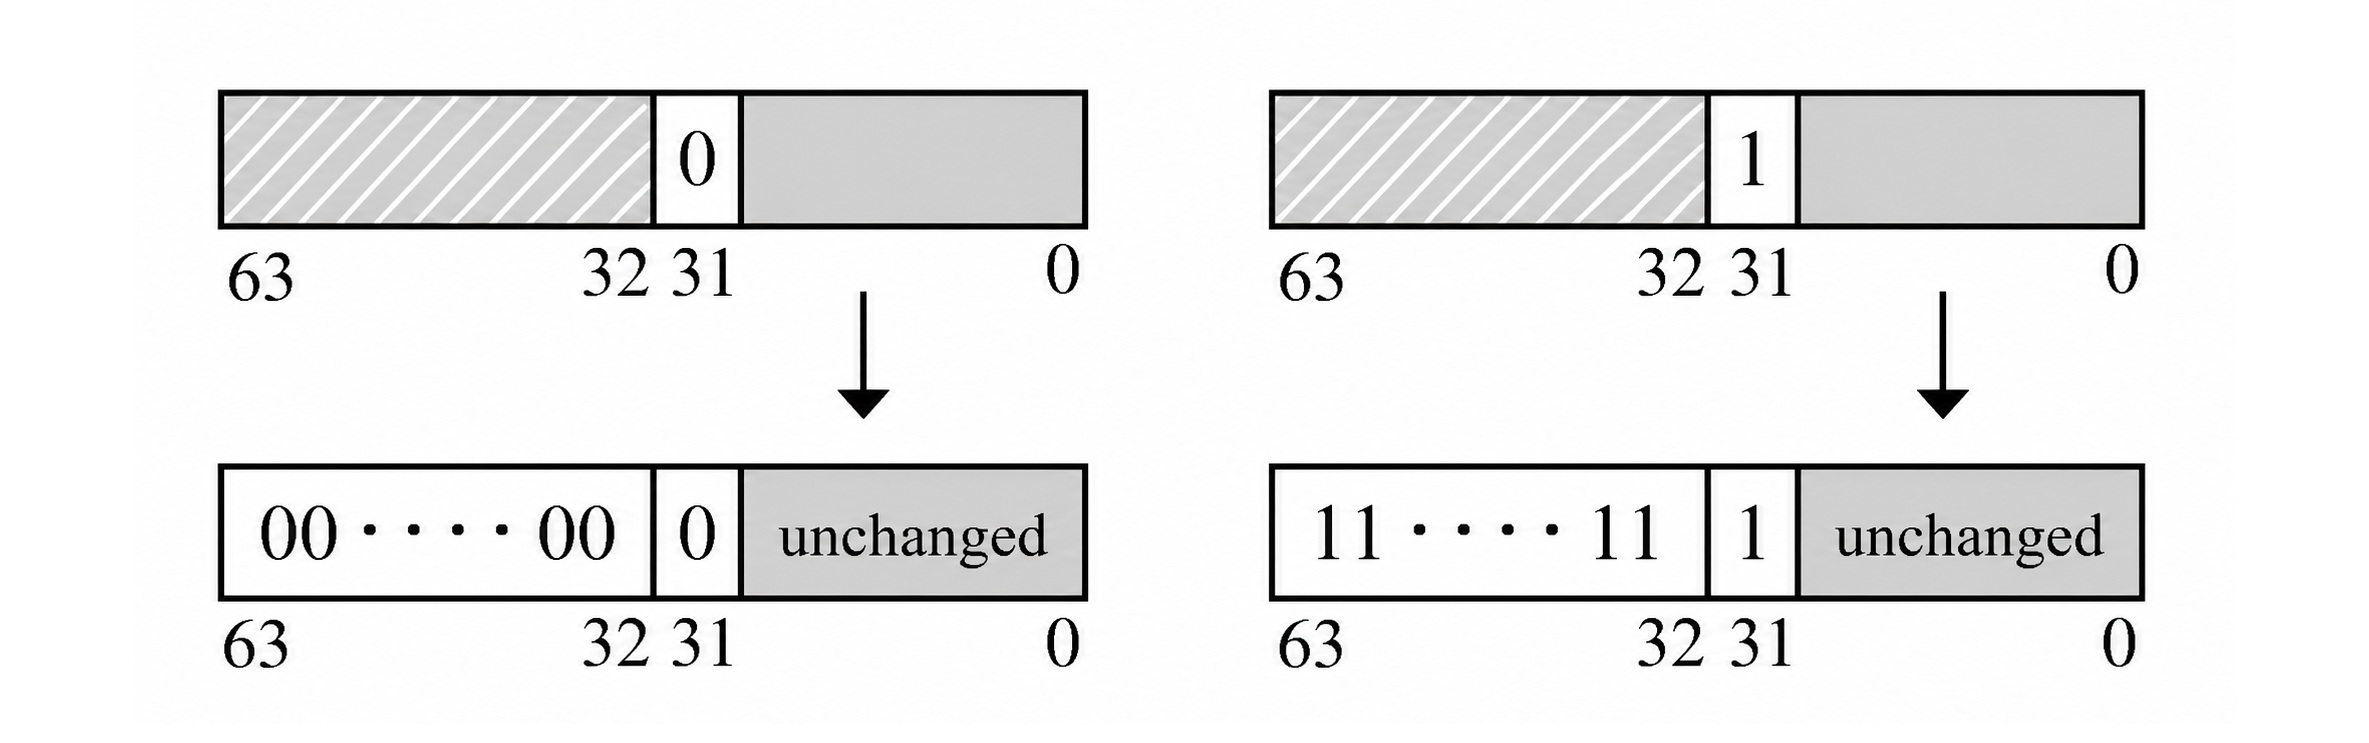
\includegraphics[width=1\columnwidth]{figures/Figure1.jpg}
  \captionsetup{justification=centering,singlelinecheck=false}
  \captionof{figure}{Sign extension of a 32-bit value to a 64-bit value.}
  \label{fig:signext-32-to-64}
\end{center}

\begin{center}
  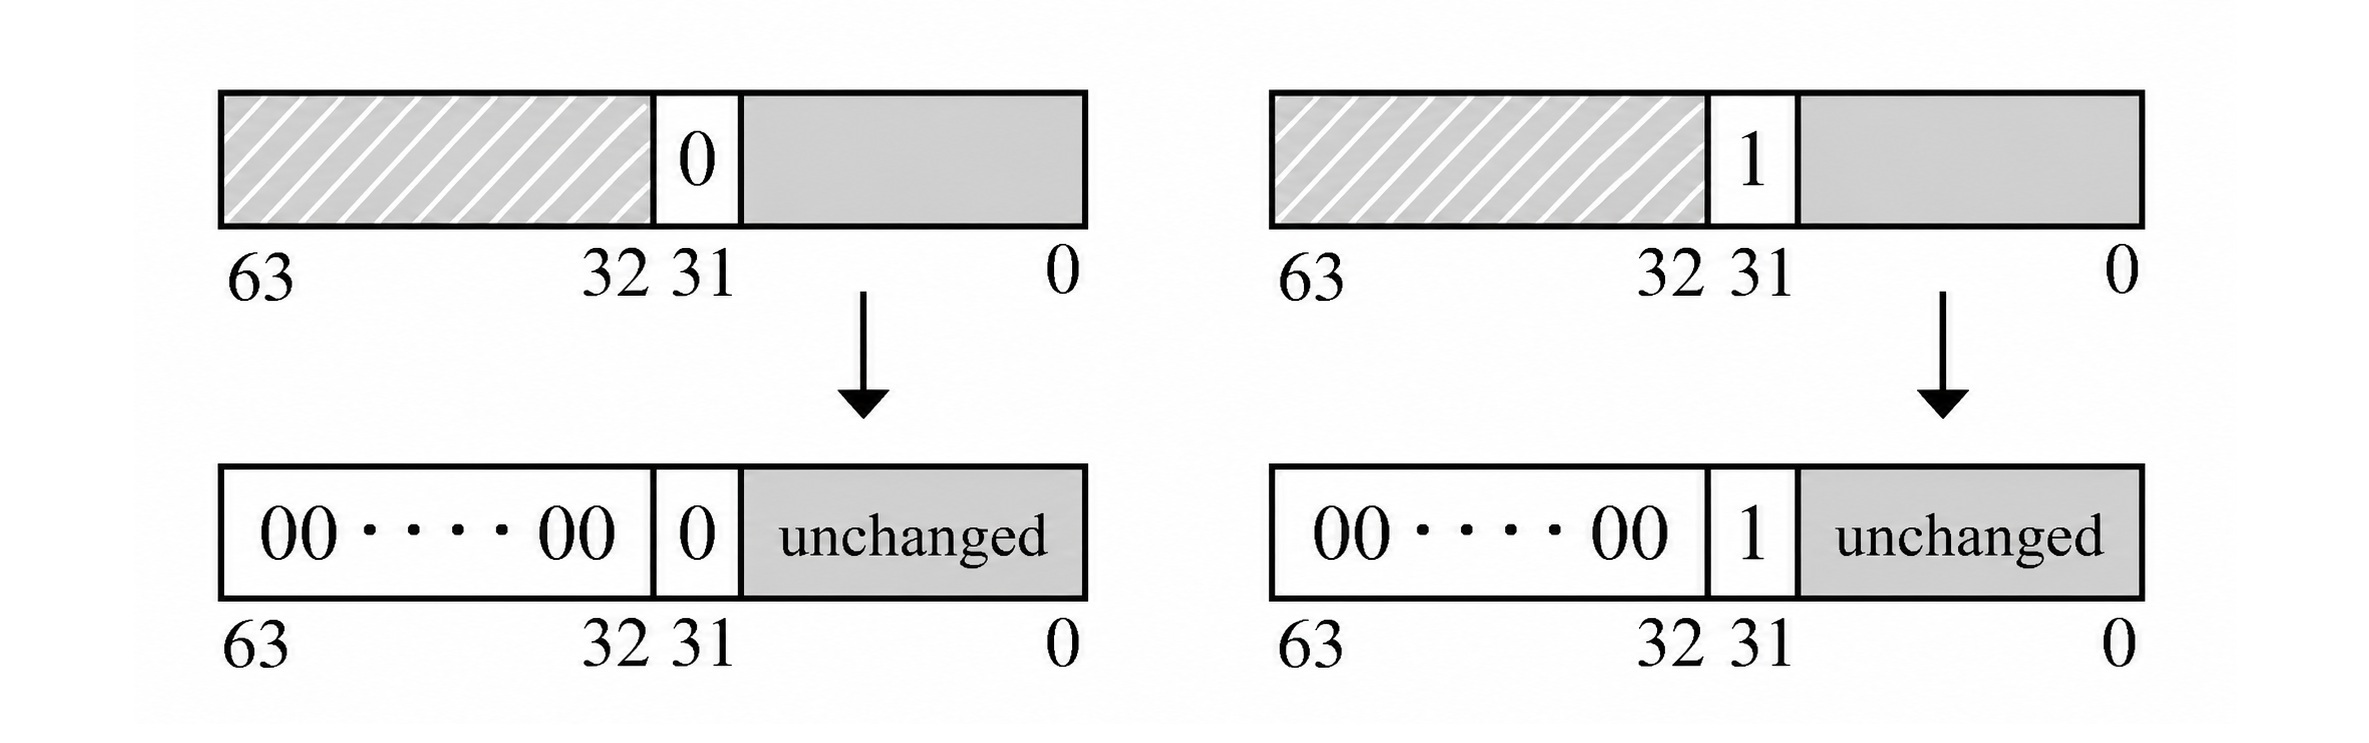
\includegraphics[width=1\columnwidth]{figures/Figure2.jpg}
  \captionsetup{justification=centering,singlelinecheck=false}
  \captionof{figure}{Zero extension of a 32-bit value to a 64-bit value.}
  \label{fig:zext-32-to-64}
\end{center}

In Figures 1 and 2, we see the two basic ways of widening a 32-bit value to 64 bits. Sign extension copies the sign bit into the new upper bits, while zero extension fills the new upper bits with zeros. Although both operations increase the bit-width of a value, they do not always preserve the same meaning. For example, the 32-bit value \texttt{0x80000000} (\texttt{-2147483648}) is negative as a signed 32-bit integer. If it is sign-extended to 64 bits, it becomes \texttt{0xFFFFFFFF80000000} and still represents \texttt{-2147483648}. If the same value is zero-extended instead, it becomes \texttt{0x0000000080000000}, which is interpreted as the positive 64-bit value \texttt{2147483648}. This is why the distinction between sign extension and zero extension becomes important during optimization and code generation.

In most architectures compiled through LLVM, register values are treated as zero-extended by default. As a result, middle-end optimizations 
tend to convert \texttt{sext} instructions into \texttt{zext}, and front-end authors are encouraged to prefer \texttt{zext} over \texttt{sext}. 
This means that by the time we see the IR, many extensions that were originally sign extensions have already been rewritten as zero extensions, 
even when this can no longer be proven from the IR alone. This becomes relevant on RISC-V RV64, where sign extension from 32 to 64 bits is often free, 
while zero extension is not~\cite{karouzakis2025llvm,riscv-isa}.



Motivated by the above, we adapt the algorithm of Kawahito et al.~\cite{kawahito2002effective}, proposed in 2002 for a Java Just-in-Time compiler targeting IA-64, to LLVM's SSA-based IR~\cite{llvm-langref}, targeting RISC-V RV64.
The algorithm inserts extensions at definition points and then selectively eliminates them, starting from the most frequently executed regions of the program. In our implementation, the adaptation is organized around the following main ideas:

\begin{itemize}
\item[--] To test the approach, we implemented two function passes for translating the program to 64-bit and effectively eliminating redundant extension instructions.
\item[--] We evaluated our results using LLVM's test suite and the MiBench benchmarks.
\end{itemize}




\section{Implementation}
\noindent Our implementation follows the structure of Kawahito et al. and adapts the algorithm to LLVM IR for RV64 as we metioned in the previous section. The optimization is performed in several stages, starting from the preparation of the IR and ending with the elimination of redundant extension instructions. The algorithm consists of four main phases:

\begin{itemize}
\item[--] translating the program's intermediate representation to a 64-bit
  architecture by widening instructions to 64 bits;
\item[--] inserting extra sign extensions before every instruction that requires
  a sign-extended operand;
\item[--] determining the elimination order, starting from the most frequently
  executed regions;
\item[--] eliminating redundant sign extensions using UD/DU chains.
\end{itemize}
The following sections describe each phase of the implementation in more detail.

\subsection{Widening}

The first phase translates the intermediate representation of the program from a 32-bit architecture form to a 64-bit architecture form by widening 32-bit (or narrower) instructions to 64 bits. To preserve the correct semantics of each instruction, truncation and sign-extension operations are inserted when necessary. This is required because a widened 64-bit instruction does not always produce the same result as its 32-bit original value. By truncating the result back to 32 bits and then sign-extending it to 64 bits, the original 32-bit behavior is preserved while allowing the value to remain in the widened representation.

This transformation is essential for sign-extension elimination. In order to eliminate a sign-extension instruction, a widened version of its source value must be available so that its users can be rewritten. Furthermore, the widened representation is required by the order-determination phase, which is described in a later section.

\begin{figure}[H]
\centering

\begin{minipage}{1\linewidth}

\textbf{Original program}

\begin{lstlisting}[
  basicstyle=\ttfamily\normalsize,
  columns=fullflexible,
  keepspaces=true,
  aboveskip=0.3em,
  belowskip=0.8em
]
1: x = sub  i32 a, b
2: y = add  i32 x, c
3: s = sext i32 y to i64
4: z = or   i64 s, -50
5: t = and  i64 s, 214
\end{lstlisting}

\textbf{After widening}

\medskip

\noindent
\begin{minipage}[t]{0.58\linewidth}
\vspace{-0.4cm}
\textnormal{(before elimination)}

\begin{lstlisting}[
  basicstyle=\ttfamily\normalsize,
  columns=fullflexible,
  keepspaces=true,
  aboveskip=0.3em,
  belowskip=0pt
]
 1: x.w   = sub   i64 a.w, b.w
 2: x.t   = trunc i64 x.w to i32
 3: x.s   = sext  i32 x.t to i64
 4: y.w   = add   i64 x.s, c.w
 5: y.t   = trunc i64 y.w to i32
 6: y.s   = sext  i32 y.t to i64
 7: y.s.t = trunc i64 y.s to i32
 8: s     = sext  i32 y.t to i64
 9: z     = or    i64 s, -50
10: t     = and   i64 s, 214
\end{lstlisting}
\end{minipage}%
\hspace{0cm}
\begin{minipage}[t]{0.36\linewidth}
\vspace{-0.4cm}
\textnormal{(after elimination)}

\begin{lstlisting}[
  basicstyle=\ttfamily\normalsize,
  columns=fullflexible,
  keepspaces=true,
  aboveskip=0.3em,
  belowskip=0pt
]
1: x.w = sub i64 a.w, b.w
2: y.w = add i64 x.w, c.w
3: z   = or  i64 y.w, -50
4: t   = and i64 y.w, 214
\end{lstlisting}
\end{minipage}

\end{minipage}

\vspace{1.2em}

\captionsetup{
  font=small,
  justification=centering,
  singlelinecheck=false,
  skip=0pt
}
\caption{Example of widening followed by sign-extension elimination.}
\label{fig:figure3}

\end{figure}

\subsection{Sign Extension Insertion}

In this phase, we insert sign-extension instructions at use points to improve sign-extension elimination in frequently executed regions such as loops. After the original sign-extension instruction, we insert a truncation and a new sign extension before the first user in the same basic block. This additional sign-extension instruction acts as a helper, allowing the extension to be moved closer to its uses and increasing the chances of eliminating sign extensions that appear inside frequently executed basic blocks.

\begin{figure}[H]
\centering

\begin{minipage}{0.88\textwidth}
\raggedright

\textbf{Sign-extension insertion}

\medskip

\noindent
\begin{minipage}[t]{0.43\linewidth}
\textnormal{(a) Before insertion}

\begin{lstlisting}[
  basicstyle=\ttfamily\normalsize,
  columns=fullflexible,
  keepspaces=true,
  aboveskip=0.3em,
  belowskip=0pt,
  xleftmargin=0pt,
  xrightmargin=0pt
]
hot_BB:
1: i = or   i64 j, k
2: x = add  i64 v, i
3: y = sub  i64 x, 255
4: s = sext i32 y to i64

cold_BB:
5: y = mul  i64 s, 155
6: z = or   i64 y, 400
\end{lstlisting}
\end{minipage}%
\hfill
\begin{minipage}[t]{0.53\linewidth}
\textnormal{(b) After insertion}

\begin{lstlisting}[
  basicstyle=\ttfamily\normalsize,
  columns=fullflexible,
  keepspaces=true,
  aboveskip=0.3em,
  belowskip=0pt,
  xleftmargin=0pt,
  xrightmargin=0pt
]
hot_BB:
1: i     = or    i64 j, k
2: x     = add   i64 v, i
3: y     = sub   i64 x, 255
4: s     = sext  i32 y to i64

cold_BB:
5: s.t   = trunc i64 y to i32
6: s.t.s = sext  i32 s.t to i64
7: y     = mul   i64 s.t.s, 155
8: z     = or    i64 y, 400
\end{lstlisting}
\end{minipage}

\end{minipage}

\captionsetup{
  font=small,
  justification=centering,
  singlelinecheck=false,
  skip=0pt
}
\vspace{1.2em}
\caption{Example of sign-extension insertion.}
\label{fig:figure4}

\end{figure}
\begin{figure}[H]
\centering
\begin{minipage}{0.64\textwidth}

\textbf{(b) Optimized result}\\[-0.2em]
\textbf{    with insertion}\\[0.05em]

\begin{lstlisting}[
  basicstyle=\ttfamily\normalsize,
  aboveskip=0pt,
  belowskip=0pt,
  columns=fullflexible,
  keepspaces=true
]
1: i     = or    i64 j, k
2: x     = add   i64 v, i
3: y     = sub   i64 x, 255

cold_BB:
4: s.t.s = sext  i64 y to i64
5: y     = mul   i64 s.t.s, 155
6: z     = or    i64 y, 400
\end{lstlisting}


\captionsetup{
  font=small,
  justification=centering,
  singlelinecheck=false,
  skip=0pt
}
\vspace{1.2em}

\caption{Optimized result with sign-extension insertion.}
\label{fig:figure5}

\end{minipage}

\end{figure}

Figures 4 and 5 show how sign-extension insertion works. In this example, the users of the \texttt{sext} instruction ((\textbf{4a}) - \textbf{line 4}) are located in a less frequently executed (\textbf{colder}) basic block. For this reason, an additional \texttt{sext} is inserted in the cold block ((\textbf{4b}) - \textbf{line 6}), while the original value can be used in the most frequently execute (\textbf{hot}) path. As a result, the most frequently executed \texttt{sext} is removed from the hot basic block and moved to a colder one. Although the sign extension cannot be completely eliminated in this case, the optimization reduces its cost by keeping it only in the less frequently executed code.

\subsection{Order Determination for Elimination}

Sign extensions should be eliminated starting from the most frequently executed regions. Otherwise, eliminating sign extensions in less frequently executed basic blocks first may reduce the opportunities for eliminating sign extensions effectively.

In the example shown in Figure 4(b), if we eliminate first the \texttt{sext} instruction of the less frequently basic block (\texttt{cold\_BB}), the \texttt{sext} of the most frequenty executed basic block (\texttt{hot\_BB}) will still be required. In this case, even though one sign-extension instruction is eliminated, the optimization does not achieve the maximum benefit because the remaining \texttt{sext} is executed more frequently.

\par\medskip
\begin{center}
\begin{minipage}{1\textwidth}

\noindent\begin{minipage}[t]{0.52\linewidth}
\raggedright
\textbf{Before elimination(Widened)}\\[0.15em]
\begin{lstlisting}[basicstyle=\ttfamily\normalsize,aboveskip=0pt,belowskip=0pt]
cold_BB:
1: x     = add   i64 i , k
2: y     = sub   i64 x , 255
3: y.t   = trunc i64 y to i32
4: y.s   = sext  i32 y.t to i64

hot_BB:
5: y.s.t = trunc i64 y.s to i32
6: y.s.s = sext  i32 y.s.t to i64
7: m     = mul   i32 y.s.s, 455

\end{lstlisting}
\end{minipage}

\vspace{0.7em}

\noindent\begin{minipage}[t]{0.48\linewidth}
\raggedright
\textbf{Optimized Result 1}\\[0.15em]
\begin{lstlisting}[basicstyle=\ttfamily\normalsize,aboveskip=0pt,belowskip=0pt]
cold_BB:
1: x   = add   i64 i , k
2: y   = sub   i64 x , 255
3: y.t = trunc i64 y to i32
4: y.s = sext  i32 y.t to i64

hot_BB:
5: m   = mul   i32 y.s, 455
\end{lstlisting}
\end{minipage}%
\hfill%
\begin{minipage}[t]{0.48\linewidth}
\raggedright
\textbf{Optimized Result 2}\\[0.15em]
\begin{lstlisting}[basicstyle=\ttfamily\normalsize,aboveskip=0pt,belowskip=0pt]
cold_BB:
1: x     = add   i64 i , k
2: y     = sub   i64 x , 255

hot_BB:
3: y.s.t = trunc i64 y to i32
4: y.s.s = sext  i32 y.s.t to i64
5: m     = mul   i32 y.s.s, 45
\end{lstlisting}
\end{minipage}

\par\vspace{1.2em}
\refstepcounter{figure}\label{fig:figure6}
\noindent\makebox[\linewidth][c]{\normalfont\small\textbf{Figure~\thefigure.} Example requiring order determination}
\par\vspace{0.6em}

\end{minipage}
\end{center}
\par\medskip

Another example is shown in Figure 6. There are two \texttt{sext} candidates for elimination(\textbf{lines 4 - 5}). Although only one of them can be eliminated, \textbf{Optimized Result 1} is clearly better than \textbf{Optimized Result 2}.

To achieve this, we sort the basic blocks from the most frequently executed to the least frequently executed, allowing us to eliminate sign-extension instructions in the correct order and prioritize the hottest regions.

\subsection{Sign Extension Elimination}

Sign extensions are analyzed and eliminated in order of execution frequency, starting from the most frequently executed regions, as described in Section 2.3.

Our elimination approach, based on the algorithm proposed by Kawahito et al., consists of two main algorithms: \texttt{EliminateOneExtend} and \texttt{AnalyzeUSE}.

\par\vspace{1.2em}

\begin{center}
\begin{minipage}{0.52\textwidth}

\begin{lstlisting}[
basicstyle=\normalfont\fontsize{9.5pt}{11pt}\selectfont,
aboveskip=0pt,
belowskip=0pt,
columns=fullflexible,
keepspaces=true,
breaklines=false
]
1: EliminateOneExtend(EXT) {
2:   initialize flags for all instructions;
3:   required = FALSE;
4:
5:   /* use DU-chain */
6:   for (I in all instructions that use
7:        the destination operand of EXT) {
8:     required = AnalyzeUSE(EXT, I, TRUE);
9:     if (required) break;
10:  }
11:
12:  if (!required)
13:    eliminate EXT;
14: }
\end{lstlisting}

\end{minipage}
\end{center}

\vspace{0.8em}

\refstepcounter{figure}\label{fig:figure7}

\begin{center}
\small\textbf{Figure~\thefigure.} The EliminateOneExtend algorithm.
\end{center}

\par\vspace{1.2em}
\par\vspace{1.2em}

\begin{center}
\begin{minipage}{0.52\textwidth}

\begin{lstlisting}[
basicstyle=\normalfont\fontsize{9.5pt}{11pt}\selectfont,
aboveskip=0pt,
belowskip=0pt,
columns=fullflexible,
keepspaces=true,
breaklines=false
]
1: AnalyzeUSE(EXT, I) {
2:   if (a flag of USE for I
3:       has already been set)
4:     return FALSE;
5:
6:   set a flag of USE for I;
7:
8:   switch(I) {
9:   case 1:
10:     /* The source operand of I does not require
11:        type S */
12:     return FALSE;
13:
14:   case 2:
15:     /* Requirement of type S of source
16:        operand of I is equal to that
17:        of the destination operand of I*/
18:
19:     /* use DU-chain */
20:     for (J in all instructions that use
21:          the destination operand of I) {
22:       if (AnalyzeUSE(EXT, J))
23:         return TRUE;
24:     }
25:
26:     return FALSE;
27:   }
28:
29:   return TRUE;
30: }
\end{lstlisting}

\end{minipage}
\end{center}

\vspace{0.8em}

\refstepcounter{figure}\label{fig:figure8}

\begin{center}
\small\textbf{Figure~\thefigure.} The AnalyzeUSE algorithm.
\end{center}

\par\vspace{1.2em}

The \texttt{EliminateOneExtend} function processes every \texttt{sext} and \texttt{zext} instruction in the program, including extensions narrower than 32 bits. For each extension instruction, it runs the \texttt{AnalyzeUSE} algorithm on all instructions that use the extension (DU-chain). If \texttt{AnalyzeUSE} returns \texttt{TRUE}, the extension is considered necessary for the instruction I and is not eliminated.

The \texttt{AnalyzeUSE} algorithm analyzes all users of the instruction that is being examined and handles two different cases. In the first case, we check if an instruction \texttt{I} does not require sign or zero extension information from its source operand. In this case, the algorithm returns \texttt{FALSE}, which means that this use path does not require the extension instruction that we are analyzing. In the second case, the algorithm cannot tell whether the source operand requires sign or zero extension. Therefore, it continues the analysis by running \texttt{AnalyzeUSE} again for all users of instruction \texttt{I} until it finds one (or not) in the path.

Instructions that can be handled by the second case are instructions where the higher bits do not affect the lower bits, such as \texttt{add}, \texttt{sub}, \texttt{and}, \texttt{or}, \texttt{xor}, \texttt{phi}, and \texttt{shl}. For these instructions, if the higher bits of their operands are not required, their behavior on the lower bits remains unchanged.

The first case includes instructions that can provide information about the higher bits of a value. Examples are instructions \texttt{'trunc'}, \texttt{'and'} with a positive constant operand, and \texttt{'or'} with an operand whose higher bits and sign bit are set to 1. Using this information, the algorithm can conclude that the higher bits are not needed. As a result, the extension instruction being analyzed is not required and can be eliminated because none of the instructions in its use path use the higher bits.

\par\vspace{1.2em}
\begin{center}
\hspace*{0.8cm}
\begin{minipage}{0.90\textwidth}

%==================== TOP ROW ====================

\begin{minipage}[t]{0.46\linewidth}
\raggedright

{\ttfamily\normalsize
\textbf{(a) Before elimination}\par}

\begin{lstlisting}[
basicstyle=\ttfamily\normalsize,
aboveskip=0pt,
belowskip=0pt,
columns=fullflexible,
keepspaces=true,
breaklines=false
]
1: x = add   i64 i, j
2: t = trunc i64 x to i32
3: s = sext  i32 t to i64
4: m = mul   i64 s, -100
5: v = and   i64 m, 255
6: z = or    i64 s, -55
\end{lstlisting}

\end{minipage}
\hfill
\begin{minipage}[t]{0.46\linewidth}
\raggedright

{\ttfamily\normalsize
\textbf{(b) Before elimination}\par}

\begin{lstlisting}[
basicstyle=\ttfamily\normalsize,
aboveskip=0pt,
belowskip=0pt,
columns=fullflexible,
keepspaces=true,
breaklines=false
]
1: x = add   i64 i, j
2: t = trunc i64 x to i32
3: s = sext  i32 t to i64
4: m = sub   i64 s, -100
5: v = and   i64 m, 255
6: z = or    i64 s, -55

\end{lstlisting}

\end{minipage}

\vspace{1.0em}

%==================== BOTTOM ROW ====================

\begin{minipage}[t]{0.46\linewidth}
\raggedright

{\ttfamily\normalsize
\textbf{(a) After elimination}\par}

\begin{lstlisting}[
basicstyle=\ttfamily\normalsize,
aboveskip=0pt,
belowskip=0pt,
columns=fullflexible,
keepspaces=true,
breaklines=false
]
1: x = add   i64 i, j
2: t = trunc i64 x to i32
3: s = sext  i32 t to i64
4: m = mul   i64 s, -100
5: v = and   i64 m, 255
6: z = or    i64 s, -55

\end{lstlisting}

\end{minipage}
\hfill
\begin{minipage}[t]{0.46\linewidth}
\raggedright

{\ttfamily\normalsize
\textbf{(b) After elimination}\par}

\begin{lstlisting}[
basicstyle=\ttfamily\normalsize,
aboveskip=0pt,
belowskip=0pt,
columns=fullflexible,
keepspaces=true,
breaklines=false
]
1: x = add   i64 i, j
2: m = sub   i64 x, -100
3: v = and   i64 m, 255
4: z = or    i64 x, -55

\end{lstlisting}

\end{minipage}

\end{minipage}
\end{center}

\refstepcounter{figure}\label{fig:figure9}

\begin{center}
\small\textbf{Figure~\thefigure.} Example of AnalyzeUSE.
\end{center}

\par\vspace{1.2em}

In Figure 9, we can see two different elimination cases. In \textbf{After Elimination (a)}, the \texttt{sext} instruction cannot be eliminated because its use path contains a \texttt{mul} instruction, where the higher bits may affect the result, even if the remaining use paths eventually reach \texttt{and}/\texttt{or} masks(case 1). Therefore, \texttt{AnalyzeUSE} stops the analysis and keeps the extension. In \textbf{After Elimination (b)}, the \texttt{sext} instruction follows a safe use path and can be eliminated. The \texttt{and} instruction with the positive constant value 255 guarantees that the higher bits are not needed, allowing the extension to be removed. Similarly, an \texttt{or} instruction with a negative constant operand, such as -55, guarantees that the higher bits are already set to the required sign-extension pattern and therefore do not require the original extension instruction.


\subsection{Design}

The implementation consists of two LLVM IR function passes~\cite{llvm-project,llvm-writing-pass}. The first pass includes the widening and sign-extension insertion phases described in Sections 2.1 and 2.2. We first identify all paths that contain \texttt{sext} and \texttt{zext} instructions. Then we promote the relevant instructions to 64 bits and insert the required \texttt{trunc} and \texttt{sext} instructions to preserve the original program semantics. After widening, we perform sign-extension insertion as described in the previous section. If the users of an extension instruction are located in a different basic block, we insert an additional \texttt{sext} or \texttt{zext} instruction at the use point. This allows the extension to be moved between basic blocks and increases the opportunities for elimination in frequently executed regions.

The second pass contains the remaining phases of the optimization. First, we sort all basic blocks according to their execution frequency, from the most frequently executed to the least frequently executed. Then we collect all \texttt{sext} and \texttt{zext} instructions into a list and run the \texttt{EliminateOneExtend} algorithm for each extension instruction in that order. This allows us to eliminate redundant extensions starting from the hottest regions of the program. Although we prioritize the elimination of \texttt{zext} instructions over \texttt{sext} instructions, because RISC-V sign extensions are often free as discussed in Section 1, the algorithm is able to eliminate both redundant \texttt{zext} and \texttt{sext} instructions.


\section{Evaluation}

For the evaluation of our approach, we use benchmarks from the LLVM Test suite and the MiBench suite. The metrics considered are code size and dynamic instruction count for the O3 and Oz optimization levels targeting the RISC-V RV64 architecture. We mainly focus on the O3 optimization level, since it applies aggressive optimizations with the goal of improving execution performance and is therefore the most relevant setting for evaluating our approach. The Oz results are also included to provide a comparison with an optimization level that focuses on reducing code size.

Initially, all benchmark programs are compiled for the RV64 target and the generated code size is measured. Then, for each benchmark, we collect the dynamic instruction count using Spike~\cite{spike-chipyard,spike-github}, the official RISC-V ISA simulator. The programs are executed on Spike together with the Proxy Kernel (pk)~\cite{riscv-pk-github}, which provides a simple runtime environment and handles the system calls required by the benchmarks. The dynamic instruction count is used to evaluate the effect of our approach on the executed code and to compare it against the baseline compilation.


\par\vspace{1.2em}

\begin{center}
{\normalfont\normalsize
\setlength{\tabcolsep}{5pt}
\renewcommand{\arraystretch}{1.08}
\begin{tabular}{@{}lrrr@{}}
\toprule
Benchmark & Original & Optimized & Pct Change \\
\midrule
sqlite3    & 685754  & 684863  & -0.12\% \\
ALAC-decode & 719583 & 719510  & -0.01\% \\
SPASS      & 557005  & 556370  & -0.11\% \\
ldecod     & 544915  & 544692  & -0.04\% \\
lencod     & 810885  & 810569  & -0.039\% \\
oggenc     & 494037  & 494002  & -0.0071\% \\
lua        & 779212  & 779228  & +0.0021\% \\
kimwitu++  & 2315055 & 2315495 & +0.019\% \\
\bottomrule
\end{tabular}
}
\end{center}

\vspace{0.12em}

\refstepcounter{figure}\label{fig:figure10}

\begin{center}
\small\textbf{Figure~\thefigure.} Code size results for llvm-test-suite at Oz.
\end{center}

\par\vspace{1.2em}

\par\vspace{1.2em}

\begin{center}
{\normalfont\normalsize
\setlength{\tabcolsep}{5pt}
\renewcommand{\arraystretch}{1.08}
\begin{tabular}{@{}lrrr@{}}
\toprule
Benchmark & Original & Optimized & Pct Change \\
\midrule
sqlite3 & 818506 & 818618 & +0.013\% \\
ALAC-decode & 723854 & 723854 & +0.00\% \\
SPASS & 622074 & 620326 & -0.28\% \\
ldecod & 595796 & 595944 & +0.024\% \\
lencod & 948404 & 948676 & +0.028\% \\
oggenc & 511426 & 511390 & -0.007\% \\
lua & 806083 & 806095 & +0.0014\% \\
kimwitu++ & 2394819 & 2394783 & -0.015\% \\
\bottomrule
\end{tabular}
}
\end{center}

\vspace{0.12em}

\refstepcounter{figure}\label{fig:figure11}

\begin{center}
\small\textbf{Figure~\thefigure.} Code size results for llvm-test-suite at O3.
\end{center}

\par\vspace{1.2em}

\par\vspace{1.2em}

\begin{center}
{\normalfont\normalsize
\setlength{\tabcolsep}{5pt}
\renewcommand{\arraystretch}{1.08}
\begin{tabular}{@{}lrrr@{}}
\toprule
Benchmark & Original & Optimized & Pct Change \\
\midrule
sqlite3      & 1191072934 & 1192664153 & +0.13\% \\
ALAC-decode  & 112174248  & 112174397  & +0.0001\% \\
SPASS        & 2995196    & 2993580    & -0.054\% \\
ldecod       & 1448596    & 1448624    & +0.0019\% \\
lencod       & 1778874    & 1779320    & +0.025\% \\
oggenc       & 3367611    & 3367749    & +0.0041\% \\
lua          & 49293168   & 49293252   & +0.0002\% \\
kimwitu++    & 88034614   & 87982278   & -0.059\% \\
\bottomrule
\end{tabular}
}
\end{center}

\vspace{0.12em}

\refstepcounter{figure}\label{fig:figure12}

\begin{center}
\small\textbf{Figure~\thefigure.} Dynamic instruction counts for llvm-test-suite at Oz.
\end{center}

\par\vspace{1.2em}

\par\vspace{1.2em}

\begin{center}
{\normalfont\normalsize
\setlength{\tabcolsep}{5pt}
\renewcommand{\arraystretch}{1.08}
\begin{tabular}{@{}lrrr@{}}
\toprule
Benchmark & Original & Optimized & Pct Change \\
\midrule
sqlite3 & 1056095684 & 1056095811 & +0.000012\% \\
ALAC-decode & 78642830 & 78642692 & -0.00017\% \\
SPASS & 2414285 & 2386430 & -1.15\% \\
ldecod & 1038120 & 1033004 & -0.49\% \\
lencod & 1034752 & 1033989 & -0.073\% \\
oggenc & 2973349 & 2973522 & +0.0058\% \\
lua & 47878251 & 47879061 & +0.0016\% \\
kimwitu++ & 83857308 & 83833604 & -0.028\% \\
\bottomrule
\end{tabular}
}
\end{center}

\vspace{0.12em}

\refstepcounter{figure}\label{fig:figure13}

\begin{center}
\small\textbf{Figure~\thefigure.} Dynamic instruction counts for llvm-test-suite at O3.
\end{center}

\par\vspace{1.2em}


The results for the LLVM Test Suite show that our transformation has a small impact on code size, while some changes can also be observed in the dynamic instruction counts.

Looking at the O3 results first, the code size remains very close to the original version for all benchmarks. The changes are generally small, with SPASS showing the largest reduction (-0.28\%). For the remaining benchmarks, the differences are very close to zero. Overall, the transformation has a very limited impact on code size.

The dynamic instruction counts show a different picture. While some benchmarks remain almost unchanged, SPASS, ldecod and lencod show reductions in the number of executed instructions, with SPASS achieving a reduction of more than 1.1\%. Across all benchmarks, the average reduction is approximately 0.22\%. One reason for this is that some extension operations are moved away from frequently executed paths and into regions that are executed less often. Because of this, fewer extension-related instructions are executed at runtime, which helps reduce the overall dynamic instruction count.

For Oz, the changes remain small overall. Several benchmarks show slight reductions in code size, which is in line with the goal of Oz optimizations. On the other hand, the dynamic instruction counts remain very close to the original version, with only minor changes across the benchmarks. As a result, the impact of our transformation is less noticeable under Oz than under O3.

\par\vspace{1.2em}

\begin{center}
{\normalfont\normalsize
\setlength{\tabcolsep}{5pt}
\renewcommand{\arraystretch}{1.08}
\begin{tabular}{@{}lrrr@{}}
\toprule
Benchmark & Original & Optimized & Pct Change \\
\midrule
consumer-jpeg & 621068 & 621096 & +0.0045\% \\
basicmath     & 514740 & 514740 & +0.00\% \\
madplay       & 742257 & 742509 & +0.034\% \\
toast         & 532244 & 532216 & -0.0053\% \\
dijkstra      & 520861 & 520861 & +0.00\% \\
\bottomrule
\end{tabular}
}
\end{center}

\vspace{0.12em}

\refstepcounter{figure}\label{fig:figure14}

\begin{center}
\small\textbf{Figure~\thefigure.} Code size results for MiBench at Oz.
\end{center}

\par\vspace{1.2em}

\par\vspace{1.2em}

\begin{center}
{\normalfont\normalsize
\setlength{\tabcolsep}{5pt}
\renewcommand{\arraystretch}{1.08}
\begin{tabular}{@{}lrrr@{}}
\toprule
Benchmark & Original & Optimized & Pct Change \\
\midrule
consumer-jpeg & 652624 & 652640 & +0.0024\% \\
basicmath & 515412 & 515412 & +0.00\% \\
madplay & 779321 & 779625 & +0.039\% \\
toast & 541477 & 541461 & -0.0029\% \\
dijkstra & 521293 & 521293 & +0.00\% \\
\bottomrule
\end{tabular}
}
\end{center}

\vspace{0.12em}

\refstepcounter{figure}\label{fig:figure15}

\begin{center}
\small\textbf{Figure~\thefigure.} Code size results for MiBench at O3.
\end{center}

\par\vspace{1.2em}

\par\vspace{1.2em}

\begin{center}
{\normalfont\normalsize
\setlength{\tabcolsep}{5pt}
\renewcommand{\arraystretch}{1.08}
\begin{tabular}{@{}lrrr@{}}
\toprule
Benchmark & Original & Optimized & Pct Change \\
\midrule
consumer-jpeg & 7106528   & 7107059   & +0.0075\% \\
basicmath     & 144186416 & 144186427 & +0.00\% \\
madplay       & 28826077  & 28717772  & -0.37\% \\
toast         & 18284169  & 18283679  & -0.0027\% \\
dijkstra      & 44742791  & 44742808  & +0.00\% \\
\bottomrule
\end{tabular}
}
\end{center}

\vspace{0.12em}

\refstepcounter{figure}\label{fig:figure16}

\begin{center}
\small\textbf{Figure~\thefigure.} Dynamic instruction counts for MiBench at Oz.
\end{center}

\par\vspace{1.2em}

\par\vspace{1.2em}

\begin{center}
{\normalfont\normalsize
\setlength{\tabcolsep}{5pt}
\renewcommand{\arraystretch}{1.08}
\begin{tabular}{@{}lrrr@{}}
\toprule
Benchmark & Original & Optimized & Pct Change \\
\midrule
consumer-jpeg & 6760463 & 6760931 & +0.0069\% \\
basicmath & 143167792 & 143167803 & +0.0000077\% \\
madplay & 25646601 & 25469129 & -0.692\% \\
toast & 16394788 & 16394712 & -0.00046\% \\
dijkstra & 33874230 & 33874247 & +0.00005\% \\
\bottomrule
\end{tabular}
}
\end{center}

\vspace{0.12em}

\refstepcounter{figure}\label{fig:figure17}

\begin{center}
\small\textbf{Figure~\thefigure.} Dynamic instruction counts for MiBench at O3.
\end{center}

\par\vspace{1.2em}


The MiBench results show a similar behavior to the one observed in the LLVM Test Suite. The impact of our transformation on code size remains small, while the dynamic instruction count results provide some additional insight into its effect on the generated code.

For the O3 setting, code size remains very close to the original version for all benchmarks. The largest increase is observed in madplay (+0.039\%), while toast shows a small reduction (-0.0029\%). The remaining benchmarks are practically unchanged. Overall, the differences in code size are very small.

The dynamic instruction counts show a similar pattern. Most benchmarks remain almost unchanged, while madplay shows the largest reduction, reaching approximately 0.69\%. This is particularly interesting because the same benchmark shows a very small increase in code size. This highlights one of the main ideas behind our implementation: a small change in code size does not necessarily translate to more instructions being executed at runtime. Across all benchmarks, the average reduction in dynamic instruction count is around 0.14\%.

For the Oz setting, the changes remain small for both metrics. The code size results stay very close to the original version, with only minor increases or decreases across the benchmarks. This is expected, because as mentioned earlier, Oz primarily focuses on reducing the size of the generated code.

The dynamic instruction counts also remain close to the baseline for most benchmarks. The only noticeable change is observed in madplay, which shows a reduction of approximately 0.37\%, while the remaining benchmarks are almost unchanged. Overall, the impact of our transformation under Oz is smaller than in O3, suggesting that the optimizations performed by Oz leave fewer opportunities for our approach to affect the final code.


\section{Discussion}
There are some limitations in the current implementation that affect the evaluation results. As discussed earlier, our approach performs a widening step from 32-bit to 64-bit values. This helps expose opportunities for extension elimination, but at the same time it can introduce additional extension instructions. Although many of these instructions are removed during the transformation, some of them remain in the generated code.

The main reason for this is that our implementation does not include the backward analysis phase of the original Kawahito et al. algorithm~\cite{kawahito2002effective}, called AnalyzeDEF. This phase is used to find additional extension elimination opportunities and would remove many of the extra trunc-sext instructions that remain after the widening step.

During the development of the pass, we observed that many extension elimination opportunities depend on this backward analysis. For this reason, implementing AnalyzeDEF would likely allow more redundant extension instructions to be removed. It could also create additional opportunities for moving extension operations to less frequently executed regions of the program.

Another possible improvement to the current implementation would be the use of LLVM's Demanded Bits Analysis~\cite{llvm-demandedbits}. This analysis identifies which bits of a value are actually needed by the instructions that use it and could help expose more extension elimination opportunities during the forward analysis phase. By providing more information about how values are used, it could allow the transformation to handle more cases and eliminate a larger number of redundant extension instructions.


\section{Conclusion}
As discussed in the previous section, our current implementation does not include the backward analysis phase (AnalyzeDEF) of the original Kawahito et al. algorithm. However, the evaluation results show that the approach can still provide useful results even without this part of the algorithm. Although the widening step introduces some extra instructions, the forward analysis phase is still able to eliminate many redundant extension operations. Combined with the movement of extension instructions to less frequently executed regions of the program, this helps reduce the dynamic instruction count of the generated code, even in cases where the code size does not show a similar reduction.

The evaluation results also highlight the potential of a more complete implementation. While the current implementation does not include all parts of the original Kawahito et al. algorithm, the observed reductions in dynamic instruction count show that the main ideas of the approach are already effective within LLVM IR. A more complete implementation could expose additional extension elimination opportunities and potentially lead to further improvements.

\backmatter

\bibliography{refs}

\end{document}
